\section{Стандартные задачи}
1. Найдите число $N,$ если 6 составляет $40\%$ от $N+5.$\\
2. Найдите число $N,$ если 9 составляет $75\%$ от $N+3.$\\
3. При каких натуральных $n$ значение данного выражения является целым числом: $\cfrac{2n^2+5n-5}{n+1}?$\\
4. При каких натуральных $n$ значение данного выражения является целым числом: $\cfrac{3n^2+4n-3}{n+3}?$\\
5. Сплавлено 40 г золота одной пробы и 60 г золота другой пробы и получено золото 62-й пробы. Какой пробы было золото первого и второго слитков, если при сплаве их поровну получается золото 61-й пробы?\\
6. Имеется сталь двух сортов с содержанием никеля в $5\%$ и $40\%.$ Сколько нужно взять каждого из этих сортов стали, чтобы получить 140 т стали с содержанием никеля в $30\%?$\\
7. Бассейн заполняется водой, поступающей через две трубы. Одна труба может заполнить бассейн за 12 часов, а другая --- за 20 часов. За сколько часов заполнится бассейн двумя трубами, работающими одновременно?\\
8. Вода, поступающая в первую трубу, может наполнить бассейн за 6 часов, а вода, вытекающая из второй трубы, может опорожнить его за 15 часов. За сколько часов наполнится бассейн, если обе трубы будут одновременно открыты?\\
9. Из А и В выехали два автомобиля. Первый проехал с постоянной скоростью весь путь. Второй проехал первую половину пути со скоростью, меньшей скорости первого на 13 км/ч, а вторую половину пути --- со скоростью 78 км/ч, в результате чего прибыл в В одновременно с первым автомобилем. Найдите скорость первого автомобиля, если известно, что она больше 48 км/ч. Ответ дайте в км/ч.\\
10. Из А и В выехали два автомобиля. Первый проехал с постоянной скоростью весь путь. Второй проехал первую половину пути со скоростью, меньшей скорости первого на 16 км/ч, а вторую половину пути --- со скоростью 96 км/ч, в результате чего прибыл в В одновременно с первым автомобилем. Найдите скорость первого автомобиля, если известно, что она больше 57 км/ч. Ответ дайте в км/ч.\\
11. Два печника, работая вместе, могут сложить печь за 12 часов. Если сначала один первый печник будет работать 2 часа, а затем один второй --- 3 часа, то они выполнят только $20\%$ всей работы. За сколько часов может сложить печь один первый печник?\\
12. Две бригады, работая вместе, могут закончить уборку урожая за 8 дней. Если сначала первая бригада будет работать 3 дня, а затем одна вторая --- 12 дней, то они выполнят $75\%$ всей работы. За сколько дней может закончить уборку урожая одна вторая бригада?\\
13. Велосипедист выехал с постоянной скоростью из города А в город В, расстояние между которыми равно 70 км. На следующий день он отправился обратно в А со скоростью на 3 км/ч больше прежней. По дороге он сделал остановку на 3 часа. В результате он затратил на обратный путь столько же времени, сколько на путь из А в В. Найдите скорость велосипедиста на пути из В в А. Ответ дайте в км/ч.\\
14. Велосипедист выехал с постоянной скоростью из города А в город В, расстояние между которыми равно 98 км. На следующий день он отправился обратно в А со скоростью на 7 км/ч больше прежней. По дороге он сделал остановку на 7 часов. В результате он затратил на обратный путь столько же времени, сколько на путь из А в В. Найдите скорость велосипедиста на пути из В в А. Ответ дайте в км/ч.\\
15. Имеется 10 литров 60-процентного раствора соли. Сколько литров воды надо долить, чтобы получить 40-процентный раствор соли?\\
16. В сосуд, содержащий 5 литров 12-процентного водного раствора некоторого вещества, добавили 7 литров воды. Сколько процентов составляет концентрация получившегося раствора?\\
17. Половину времени, затраченного на дорогу, автомобиль ехал со скоростью 90 км/ч, а вторую половину времени --- со скоростью 60 км/ч. Найдите среднюю скорость автомобиля на протяжении всего пути.\\
18. Первую половину пути автомобиль проехал со скоростью 90 км/ч, вторую половину пути --- со скоростью 60 км/ч. Найдите среднюю скорость автомобиля на протяжении всего пути.\\
19. Игорь и Паша могут покрасить забор за 3 часа. Паша и Володя могут покрасить этот же забор за 6 часов, Володя и Игорь --- за 4 часа. За какое время мальчики покрасят забор, работая вместе?\\
20. Маша и Настя могут вымыть окно за 20 минут. Настя и Лена могут вымыть это же окно за 15 минут, а Маша и Лена --- за 12 минут. За какое время девочки вымоют окно, работая втроём?\\
21. Мальчик сбежал вниз по движущемуся эскалатору и насчитал 20 ступенек. Затем он пробежал вверх по тому же эскалатору с той же скоростью относительно эскалатора и насчитал 60 ступенек. Сколько ступенек он насчитал бы, спустившись по неподвижному эскалатору?\\
22. Мальчик сбежал вниз по движущемуся эскалатору и насчитал 30 ступенек. Затем он пробежал вверх по тому же эскалатору с той же скоростью относительно эскалатора и насчитал 70 ступенек. Сколько ступенек он насчитал бы, спустившись по неподвижному эскалатору?\\
23. Из трёхзначного числа вычли сумму его цифр. Может ли разность быть равной 189?\\
24. Из трёхзначного числа вычли сумму его цифр. Может ли разность быть равной 180?\\
25. При каких натуральных $n$ значение выражения $\cfrac{n^2+5n-8}{n+3}$ является целым числом?\\
26. При каких натуральных $n$ значение выражения $\cfrac{-n^2+2n-31}{n+3}$ является целым числом?\\
27. Заказ на 180 деталей первый рабочий выполняет на 3 часа быстрее, чем второй. Сколько деталей в час делает второй рабочий, если известно, что первый в час делает на 3 детали больше?\\
28. Заказ на 156 деталей первый рабочий выполняет на 1 час быстрее, чем второй. Сколько деталей в час делает второй рабочий, если известно, что первый в час делает на 1 деталь больше?\\
29. В январе товар стоил 30000 рублей. В марте цену на товар подняли на $4\%,$ а в июле снизили на $4\%.$ Сколько стоил товар в июле?\\
30. В феврале товар стоил 20000 рублей. В мае цену подняли на $6\%,$ а в августе снизили
на $6\%.$ Сколько стоил товар в августе?\\
31. Расстояние между пристанями А и В равно 18 км. Из А в В по течению реки отправился плот, а через 30 мин за ним отправилась моторная лодка, которая, прибыв в пункт В, тотчас повернула обратно и возвратилась в пункт А. К этому времени плот прошёл 9 км. Найдите скорость лодки в неподвижной воде, если скорость течения реки равна 50 м/мин.\\
32. Расстояние между пристанями А и В равно 14 км. Из А в В по течению реки отправился плот, а через 44 мин за ним отправилась моторная лодка, которая, прибыв в пункт В, тотчас повернула обратно и возвратилась в пункт А. К этому времени плот прошёл 7 км. Найдите скорость лодки в неподвижной воде, если скорость течения реки равна 50 м/мин.\\
33. Один раствор содержит $20\%$ (по объёму) соляной кислоты, а второй содержит $70\%$ кислоты. Сколько литров первого и второго растворов нужно взять, чтобы получить 100 л $50\%$-го раствора соляной кислоты?\\
34. Имеется кусок сплава меди с оловом массой 15 кг, содержащий $40\%$ меди. Сколько чистого олова надо прибавить к этому куску, чтобы получившийся новый сплав содержал $30\%$ меди?\\
35. В каждом из двух ящиков лежит 15 шаров. Число синих шаров в обоих ящиках равно 8, остальные шары --- красные. Сколько красных шаров лежит в каждом ящике, если в первом ящике на каждый синий шар приходится в 2 раза меньше красных шаров, чем во втором?\\
36. В каждом из двух ящиков лежит 40 кубиков. Число жёлтых кубиков в обоих ящиках равно 14, остальные кубики --- зелёные. Сколько зелёных кубиков лежит в каждом ящике, если в первом ящике на каждый жёлтый кубик приходится в 3 раза меньше зелёных кубиков, чем во втором?\\
37. На финальной распродаже скидка на все товары составляет $50\%,$ при этом по карте магазина постоянным покупателям предоставляется дополнительная скидка $30\%.$ При каком последовательном использовании скидок итоговая скидка больше и сколько она составит в каждом случае?\\
38. На финальной распродаже скидка на все товары составляет $70\%,$ при этом по карте магазина постоянным покупателям предоставляется дополнительная скидка $20\%.$ При каком последовательном использовании скидок итоговая скидка больше и сколько она составит в каждом случае?\\
39. Перед отправкой тепловоз издал гудок с частотой $f_0=593$ Гц. Чуть позже издал гудок подъезжающий к платформе тепловоз. Из-за эффекта Допплера частота второго гудка $f$ больше первого: она зависит от скорости тепловоза по закону $f(v)=\cfrac{f_0}{1-\frac{v}{c}}$ (Гц), где $c$ --- скорость звука в м/с. Человек, стоящий на платформе, различает сигналы по тону, если они отличаются не менее, чем на 7 Гц. Определите, с какой минимальной скоростью приближался к платформе тепловоз, если человек смог различить сигналы, а $c=300$ м/с. Ответ выразите в м/с.\\
40. Перед отправкой тепловоз издал гудок с частотой $f_0=154$ Гц. Чуть позже издал гудок подъезжающий к платформе тепловоз. Из-за эффекта Допплера частота второго гудка $f$ больше первого: она зависит от скорости тепловоза по закону $f(v)=\cfrac{f_0}{1-\frac{v}{c}}$ (Гц), где $c$ --- скорость звука в м/с. Человек, стоящий на платформе, различает сигналы по тону, если они отличаются не менее, чем на 6 Гц. Определите, с какой минимальной скоростью приближался к платформе тепловоз, если человек смог различить сигналы, а $c=320$ м/с. Ответ выразите в м/с.\\
41. Из Вены в Стамбул отправился пассажирский поезд, а навстречу ему из Стамбула в Вену через 3 часа вышел товарный поезд. После встречи пассажирский поезд ехал еще 3 часа до Стамбула, а товарный ---
6 часов до Вены. Сколько часов был в пути каждый из поездов?\\
42. Из пункта А в пункт Б отправился велосипедист Вася, а через 2 минуты ему навстречу из Б в А выехал велосипедист Петя. От места встречи на дороге Вася добрался до пункта Б за 11 минут, а Петя до пункта А за 9 минут. Сколько минут был в пути каждый из них?\\
43. К краю большого квадратного листа приложили маленький квадратик, как показано на рисунке, и в результате периметр листа увеличился на $5\%.$ На сколько $\%$ увеличилась площадь листа?
\begin{figure}[h]
\center{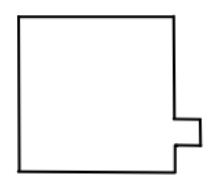
\includegraphics[scale=0.35]{2q2.png}}
\end{figure}\\
44. От края большого квадратного листа отрезали маленький квадратик, как показано на рисунке, и в результате периметр листа увеличился на $10\%.$ На сколько $\%$ уменьшилась площадь листа?
\begin{figure}[h]
\center{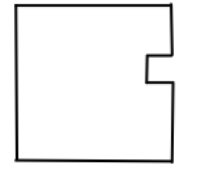
\includegraphics[scale=0.35]{1q1.png}}
\end{figure}\\
45. Из бутыли, наполненной $12\%$-ным раствором соли, отлили 1 л и долили бутыль водой, затем отлили ещё литр и опять долили водой. В бутыли оказался $3\%$-ный раствор соли. Какова вместимость бутыли?\\
46. Фляга наполнена $96\%$-ным раствором соляной кислоты. Из неё отлили 12 л кислоты и дополнили флягу водой. Затем из фляги отлили ещё 18 л и снова дополнили её водой, после чего концентрация кислоты во фляге составила $32\%.$ Найдите объём фляги.\\
47. В трёх литрах воды размешали пять чайных ложек минерального удобрения, а в десяти литрах --- две. Оба раствора слили в один бак и получили раствор удобрения нужной концентрации. Сколько чайных ложек удобрения нужно размешать в 65 литрах воды для получения раствора удобрения такой же концентрации?\\
48. Банк в конце года начисляет $20\%$ к сумме, находящейся на счёте в начале года. Каким станет вклад 50000 рублей через 3 года?\\
49. Банк в конце года начисляет $10\%$ к сумме, находящейся на счёте в начале года. Каким станет вклад 70000 рублей через 3 года?\\
50. Два велосипедиста выехали одновременно из пункта $A$ в $B,$ первый со скоростью 24 км/ч, а второй --- 18 км/ч. Спустя час вслед за ними выехал автомобиль, который обогнал второго велосипедиста на 10 минут раньше, чем первого. Найдите скорость автомобиля.\\
51. Две лодки вышли одновременно из пункта $A$ в $B,$ первая со скоростью 12 км/ч, а вторая --- 9 км/ч. Спустя час вслед за ними вышел катер, который обогнал вторую лодку на 10 минут раньше, чем первую. Найдите скорость катера.\\
52. В предвыборном штабе депутат листовки печатают 4 станка разной мощности. При печатании листовок на 1-м, 2-м и 4-м станках весь тираж будет готов за 1 час 48 мин; при печатании на 1-м, 2-м и 3-м --- за 2 часа 15 минут, а если листовки печатать на 3-м и 4-м станках, то тираж напечатают за 1,5 часа. За какое время будет готов весь тираж при совместной работе всех четырёх станков?\\
53. Автобус выехал из пункта $A$ в пункт $B.$ Не доехав 15 км до середины пути, автобус остановился для ремонта, которые занял 1 ч 30 мин. Оставшуюся часть пути автобус шёл со скоростью, на 20 км/ч больше первоначальной, и поэтому приехал в пункт $B$ вовремя. Если бы автобус весь путь шёл со скоростью, на 9 км/ч большей первоначальной, то он затратил бы на весь путь 10 ч. Найдите первоначальную скорость автобуса и расстояние между пунктами $A$ и $B.$\\
54. Автобус выехал из пункта $C$ в пункт $D.$ Проехав половину пути и ещё 40 км с постоянной скоростью, автобус остановился для ремонта, который занял 50 мин.  Оставшуюся часть пути автобус шёл со скоростью, на 5 км/ч меньшей первоначальной, и поэтому приехал в пункт $D$ с опозданием на 1 ч. Если бы автобус весь путь шёл со скоростью, на 20 км/ч меньшей первоначальной, то она затратил бы на весь путь 8 ч. Найдите первоначальную скорость автобуса и расстояние между пунктами $C$ и $D.$\\
55. Имеется два сосуда с водным раствором серной кислоты. В первом сосуде содержится 70 мл чистой кислоты, а во втором --- 60 мл. Слив содержимое этих сосудов вместе, получили 600 мл нового раствора. Найдите концентрацию кислоты в каждом из первоначальных растворов, если концентрация во втором сосуде была на $20\%$ меньше, чем в первом.\\
56. На предприятии доля сотрудников с высшим образованием составляла $80\%.$ После того как на работу было принято 30 новых специалистов с высшим образованием, доля сотрудников с высшим образованием увеличилась до $85\%.$ Сколько сотрудников теперь работает на предприятии?\\
57. Доля брака в партии изделий составляла $9\%.$ На стадии контроля качества удалось выявить и изъять из партии 40 бракованных изделий. Сколько изделий осталось в партии, если доля брака в ней составляет теперь $2,5\%?$\\
58. Два поезда выезжают одновременно из пунктов А и В навстречу друг другу. После их встречи первый прибывает в пункт В через 50 часов, а второй --- в пункт А через 8 часов. Сколько времени прошло от начала движения поездов до их встречи, если они двигались с постоянными скоростями?\\
59. Два велосипедиста выезжают одновременно из пунктов А и В навстречу друг другу. После их встречи первый прибывает в пункт В через 48 минут, а второй --- в пункт А через 27 минут. Сколько времени прошло от начала движения велосипедистов до их встречи, если велосипедисты двигались с постоянными скоростями?

ewpage
